\documentclass[11pt]{charter}
\usepackage{pdflscape}

% El títulos de la memoria, se usa en la carátula y se puede usar el cualquier lugar del documento con el comando \ttitle
\titulo{Medición y aceptación de parámetros en transformadores de corriente alterna} 

% Nombre del posgrado, se usa en la carátula y se puede usar el cualquier lugar del documento con el comando \degreename
\posgrado{Carrera de Especialización en Sistemas Embebidos} 
%\posgrado{Carrera de Especialización en Internet de las Cosas} 
%\posgrado{Carrera de Especialización en Intelegencia Artificial}
%\posgrado{Maestría en Sistemas Embebidos} 
%\posgrado{Maestría en Internet de las cosas}

% Tu nombre, se puede usar el cualquier lugar del documento con el comando \authorname
\autor{Cristian Trinidad} 

% El nombre del director y co-director, se puede usar el cualquier lugar del documento con el comando \supname y \cosupname y \pertesupname y \pertecosupname
\director{Esp. Lic. Leopoldo A. Zimperz}
\pertenenciaDirector{Iris Tecnologia S.R.L.} 
% FIXME:NO IMPLEMENTADO EL CODIRECTOR ni su pertenencia
\codirector{} % si queda vacio no se deberíá incluir 
\pertenenciaCoDirector{}

% Nombre del cliente, quien va a aprobar los resultados del proyecto, se puede usar con el comando \clientename y \empclientename
\cliente{Esp. Lic. Leopoldo A. Zimperz}
\empresaCliente{Iris Tecnologia S.R.L.}

% Nombre y pertenencia de los jurados, se pueden usar el cualquier lugar del documento con el comando \jurunoname, \jurdosname y \jurtresname y \perteunoname, \pertedosname y \pertetresname.
\juradoUno{Nombre y Apellido (1)}
\pertenenciaJurUno{pertenencia (1)} 
\juradoDos{Nombre y Apellido (2)}
\pertenenciaJurDos{pertenencia (2)}
\juradoTres{Nombre y Apellido (3)}
\pertenenciaJurTres{pertenencia (3)}
 
\fechaINICIO{22 de junio de 2020}		%Fecha de inicio de la cursada de GdP \fechaInicioName
\fechaFINALPlanificacion{22 de Agosto de 2020} 	%Fecha de final de cursada de GdP
\fechaFINALTrabajo{22 de diciembre de 2020}		%Fecha de defensa pública del trabajo final


\begin{document}

\maketitle
\thispagestyle{empty}
\pagebreak


\thispagestyle{empty}
{\setlength{\parskip}{0pt}
\tableofcontents{}
}
\pagebreak


\section{Registros de cambios}
\label{sec:registro}


\begin{table}[ht]
\label{tab:registro}
\centering

\begin{tabularx}{\linewidth}{@{}|c|X|c|@{}}
\hline
\rowcolor[HTML]{C0C0C0} 
Revisión & \multicolumn{1}{c|}{\cellcolor[HTML]{C0C0C0}Detalles de los cambios realizados} & Fecha      \\ \hline
1.0      & Creación del documento                                                          & 22/06/2020 \\ \hline
1.1      & Ejemplo de un texto muy largo que debiera ocupar más de una línea para que tengan de ejemplo                                                                                																						   & dd/mm/aaaa \\ \hline
1.2      & Otro ejemplo \newline
		   Con texto partido \newline
		   En varias líneas \newline
		   A propósito                                                                     & dd/mm/aaaa \\ \hline
\end{tabularx}
\end{table}

\pagebreak



\section{Acta de Constitución del Proyecto}
\label{sec:acta}

\begin{flushright}
Buenos Aires, \fechaInicioName
\end{flushright}

\vspace{2cm}

Por medio de la presente se acuerda con el Ing. \authorname\hspace{1px} que su Trabajo Final de la \degreename\hspace{1px} se titulará ``\ttitle'', consistirá esencialmente en el prototipo preliminar de un dispositivo capaz de medir y registrar parámetros de transformadores de corriente alterna empleados en la fabricación de dispositivos electromédicos, y tendrá un presupuesto preliminar estimado de 600 hs de trabajo y \$155237, con fecha de inicio \fechaInicioName\hspace{1px} y fecha de presentación pública \fechaFinalName.

Se adjunta a esta acta la planificación inicial.

\vfill

% Esta parte se construye sola con la información que hayan cargado en el preámbulo del documento y no debe modificarla
\begin{table}[ht]
\centering
\begin{tabular}{ccc}
\begin{tabular}[c]{@{}c@{}}Ariel Lutenberg \\ Director posgrado FIUBA\end{tabular} &  & \begin{tabular}[c]{@{}c@{}}\clientename \\ \empclientename \end{tabular} \vspace{2.5cm} \\ 
\multicolumn{3}{c}{\begin{tabular}[c]{@{}c@{}} \supname \\ Director del Trabajo Final\end{tabular}} \vspace{2.5cm} \\
\begin{tabular}[c]{@{}c@{}}\jurunoname \\ Jurado del Trabajo Final\end{tabular}     &  & \begin{tabular}[c]{@{}c@{}}\jurdosname\\ Jurado del Trabajo Final\end{tabular}  \vspace{2.5cm}  \\
\multicolumn{3}{c}{\begin{tabular}[c]{@{}c@{}} \jurtresname\\ Jurado del Trabajo Final\end{tabular}} \vspace{.5cm}                                                                     
\end{tabular}
\end{table}




\section{Descripción técnica-conceptual del Proyecto a realizar}
\label{sec:descripcion}


La empresa Iris tecnología S.R.L. fabrica equipos electromédicos cumpliendo con los requisitos de Buenas Prácticas de Fabricación exigidos por la Administración Nacional de Medicamentos, Alimentos y Tecnología Médica (A.N.M.A.T.). Adicionalmente, incorporó recientemente un sistema de gestión de calidad para fabricación de dispositivos médicos, basado en la norma ISO13485:2016. En la actualidad se está trabajando en la incorporación de tecnologías para agilizar tareas y controles que deben realizarse acorde a dicho sistema de calidad. 

Entre las tareas y controles antes mencionados se encuentra el ensayo y calificación de  transformadores para su posterior utilización en las líneas de producción. El objetivo de este proyecto es proveer un dispositivo capaz de automatizar este procedimiento que, actualmente, se realiza en forma manual. Esta labor además de insumir una gran cantidad de tiempo y ser muy repetitiva, presenta un gran riesgo de error humano, y puede además, comprometer la seguridad del operario y la fiabilidad de los datos obtenidos.

La idea es desarrollar un prototipo capaz de medir y registrar los parámetros de transformadores de tensión alterna empleados en la fabricación de dispositivos electromédicos, a fin ser aceptados o rechazados para su posterior uso. Los parámetros a medir incluyen las tensiones y corrientes de los bobinados primario y secundario.

En la Figura \ref{fig:diagBloques} se presenta el diagrama en bloques del sistema. En la figura se destaca el dispositivo a diseñar dentro del recuadro, adicionalmente se incluyen el transformador a ensayar y las fuentes de corriente alternas externas. Dentro del dispositivo a diseñar se observan los siguientes bloques principales:

\begin{itemize}
\item Módulo ESP32 con WiFi integrado.
\item Bloques de acondicionamiento de señal y actuación para el bobinado primario y secundario.
\item Interfaz de usuario: pulsadores, \textit{display} y \textit{buzzer}.
\item Interfaz para impresora RS232.
\item \textit{Switch} de seguridad para indicar que la tapa de seguridad ha sido removida.
\item Fuente de alimentación.
\end{itemize}

El dispositivo propuesto deberá indicar al operador si el transformador es aceptado o rechazado en base a umbrales previamente configurados por medio de una comunicación WiFi. Además de mostrar el resultado del ensayo localmente, este y las mediciones realizadas deberán ser enviados a un servidor web a través de la comunicación WiFi y adicionalmente se debe imprimir una etiqueta que permita la trazabilidad del componente.

A continuación se presenta un resumen de las tareas propuestas para el dispositivo a desarrollar:
\begin{itemize}
\item Mediciones de tensión y corriente a los transformadores bajo ensayo.
\item Configuración de umbrales de aceptación para los parámetros medidos.
\item Emitir confirmación de aceptación o rechazo del transformador.
\item Visualización en \textit{display} LCD de umbrales seteados y mediciones.
\item Envío de las mediciones a servidor web, vía red WiFi.
\item Impresión de etiquetas con número de partida y valores medidos. 
\end{itemize}

\begin{figure}[htpb]
\centering 
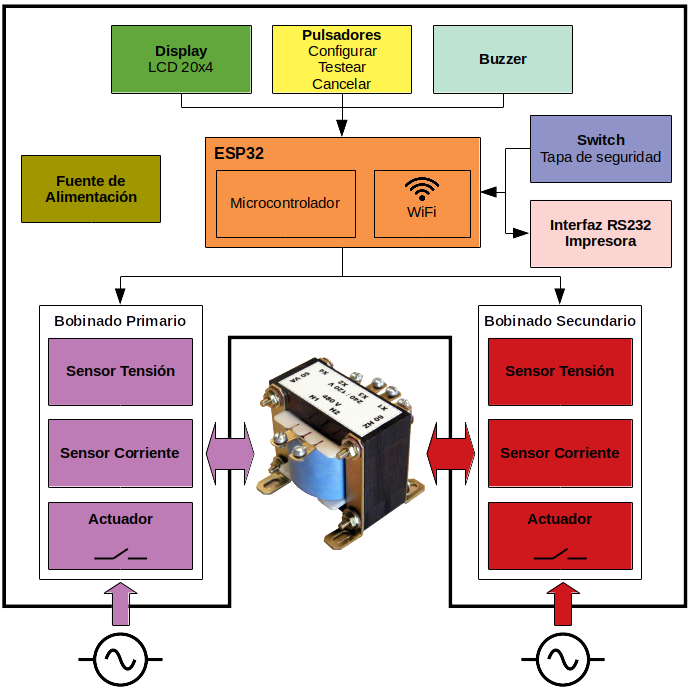
\includegraphics[width=.8\textwidth]{./Figuras/diagBloques.png}
\caption{Diagrama en bloques del sistema}
\label{fig:diagBloques}
\end{figure}

\section{Identificación y análisis de los interesados}
\label{sec:interesados}

\begin{consigna}{red} 
\begin{table}[ht]
%\caption{Identificación de los interesados}
%\label{tab:interesados}
\begin{tabularx}{\linewidth}{@{}|l|X|X|l|@{}}
\hline
\rowcolor[HTML]{C0C0C0} 
Rol           & Nombre y Apellido & Organización 	& Puesto 	\\ \hline
Cliente       & \clientename      &\empclientename	& Socio     \\ \hline
Responsable   & \authorname       & FIUBA        	& Alumno 	\\ \hline
Orientador    & \supname	      & \pertesupname 	& Director	Trabajo final \\ \hline
Usuario final & Operadores        &\empclientename	& Operador 	\\ \hline
\end{tabularx}
\end{table}
\end{consigna}



\section{1. Propósito del proyecto}
\label{sec:proposito}

El propósito de este proyecto es disminuir el riesgo de error humano y aumentar la fiabilidad de los datos obtenidos al evaluar los transformadores. Asimismo, se requiere aumentar la seguridad de los operadores expuestos a altas tensiones con la simplificación del procedimiento de caracterización y la incorporación de métodos de protección en el prototipo a diseñar.


\section{2. Alcance del proyecto}
\label{sec:alcance}

El presente proyecto tiene como alcance:
\begin{itemize}
\item Análisis, investigación y elección del hardware.
\item Investigar sobre un modelo de impresora a adquirir, cuyo protocolo esté disponible y permita llevar a cabo el proyecto.
\item Diseño e implementación del firmware del sistema en lenguaje C.
\item Desarrollo de un prototipo funcional sobre un PCB tipo universal.
\item Elaboración de un manual de usuario con la información mínima requerida para la operación del dispositivo y con las recomendaciones para evitar descargas de alta tensión. 
\end{itemize}

Queda excluido del alcance de este proyecto:
\begin{itemize}
\item El desarrollo de circuitos de medición de tensión y/o corriente alterna de precisión. Se acepta la precisión obtenida de módulos comerciales como el ZMPT101B.
\item El desarrollo de fuentes de tensión alterna para alimentar los transformadores en ensayo. El cliente deberá proporcionar al dispositivo los 230Vac estabilizados necesarios para alimentar el bobinado primario y la tensión alterna adecuada para alimentar el bobinado secundario.
\item El desarrollo de una interfaz web desde la cual interactuar por WiFi con el módulo.
\item El desarrollo del servidor web o API de colección de datos del en el servidor/PC del cliente. Esta será provista por el cliente.
\item El desarrollo de un prototipo de fabricación escalable que cumpla con todas las certificaciones necesarias.
\item El desarrollo de un PCB, más allá del prototipo en placa universal.
\item El diseño del gabinete para la instalación del sistema electrónico.
\item El diseño de circuitos de protección del operario contra descargas eléctricas de alta tensión. En este sentido, se asume que el operario que utilizará el dispositivo es idóneo en el tema. Asimismo, se asume que el cliente posee en sus instalaciones las medidas de seguridad pertinentes para el trabajo con altas tensiones, como disyuntores y puestas a tierras, acorde con la normativa vigente de Higiene y Seguridad en el Trabajo.
\end{itemize}

\section{3. Supuestos del proyecto}
\label{sec:supuestos}


Para el desarrollo del presente proyecto se supone que:

\begin{itemize}
\item La precisión necesaria para las mediciones de tensión y/o corrientes pueden ser obtenida con el uso de módulos comerciales como el ZMPT101B con modificaciones mínimas.
\item Los costos de los materiales serán cubiertos por el cliente.
\item Los materiales necesarios para el armado del prototipo pueden ser comprados en el país, aun con las restricciones de importación impuestas por el COVID-19.
\item El cliente proveerá los transformadores a medir.
\item El cliente proveerá la impresora a utilizar.
\item La impresora a utilizar posee interfaz RS-232.
\item El protocolo de la impresora a utilizar debe estar disponible para su implementación. No está contemplado dentro del proyecto hacer ingeniería inversa sobre la impresora a utilizar.
\item Si bien se incluyen algunas protecciones para el manejo de tensiones de 220 Vac, como se dijo anteriormente, se asume que el operario es idóneo y conoce los riesgos en la operación del dispositivo y que el cliente cumple las reglamentaciones de Higiene y Seguridad en el Trabajo.
\item El cliente es responsable de proporcionar, en caso de ser necesario y de una manera simple de entender e implementar, los requerimientos asociados al cumplimiento de su sistema de gestión de calidad para la fabricación de dispositivos médicos, basado en la norma ISO13485:2016 y cualquier otra normativa de cumplimiento necesario.
\end{itemize}



\section{4. Requerimientos}
\label{sec:requerimientos}


\begin{enumerate}
\item Requerimientos de hardware
	\begin{enumerate}
	\item El dispositivo debe ser diseñado en base al módulo ESP32.
	\item El dispositivo debe ser capaz de medir tensiones y corrientes alternas de manera aislada del transformador bajo ensayo.
	\item El dispositivo debe ser capaz de conmutar las tensiones primarias y secundarias.
	\item El dispositivo debe tener un \textit{display} LCD alfanumérico 20x4 caracteres.
	\item El dispositivo debe tener una interfaz Wifi.
	\item El dispositivo debe tener una interfaz RS232 capaz de manejar impresoras.
	\item El dispositivo debe alimentarse desde la red eléctrica Argentina 220Vac/50hz, debiendo proveerse todas las alimentaciones a los diferentes módulos de hardware.
	\item El dispositivo debe poseer un \textit{switch} para indicar que la tapa de seguridad ha sido removida.
	\item El dispositivo debe poseer 3 pulsadores nombrados Configurar, Testear y Cancelar.
	\item El dispositivo debe poseer un \textit{buzzer}.
	\end{enumerate}
\item Requerimientos relativos a los valores a medir
	\begin{enumerate}
	\item Bobinado primario
		\begin{enumerate}
		\item Rango tensión: 100 – 240 Vac
		\item Rango corriente: 0 – 800 mAac
		\end{enumerate}
	\item Bobinado secundario
		\begin{enumerate}
		\item Rango tensión: 0 – 30 Vac
		\item Rango corriente: 0 – 1500 mAac
		\end{enumerate}
	\item Precisión en la medición de tensión: mejor al 1,5\% (puede variar en base a lo que se pueda conseguir en el mercado)
	\item Precisión en la medición de corriente: mejor al 4\% (puede variar en base a lo que se pueda conseguir en el mercado)
	\end{enumerate}
\item Requerimientos funcionales
	\begin{enumerate}
	\item El dispositivo debe permitir que se configuren los umbrales mínimos y máximos para los parámetros medidos. 
	\item Los valores a configurar deben ser adquiridos solo por WiFi, no se admite configuración local por teclado.
	\item El dispositivo debe generar una confirmación de aceptación o rechazo del transformador en ensayo basado en los umbrales mínimos y máximos preseteados.
	\item El dispositivo, luego de cada ensayo, independientemente del resultado, debe imprimir una etiqueta con la siguiente información:
		\begin{enumerate}
		\item Número de partida del transformador ensayado
		\item Condición de aceptado o rechazado
		\item Valores medidos de tensiones y corrientes
		\end{enumerate}
	\item El dispositivo debe seguir de forma automática la siguiente secuencia de testeo básico:
		\begin{itemize}
		\item Pulsar Testear
		\item Verificar si el dispositivo fue configurado, sino pedir parámetros de configuración
		\item Energizar el bobinado primario con 230Vac estabilizados  (provistos externamente por el cliente)
		\item Medir:
			\begin{itemize}
			\item Tensión en bobinado primario
			\item Corriente que circula por el bobinado primario
			\item Tensión en bobinado secundario
			\end{itemize}
		\item Desenergizar el bobinado primario
		\item Energizar el bobinado secundario con la tensión adecuada (provista externamente por el cliente)
		\item Medir:
			\begin{itemize}
			\item Tensión en bobinado primario
			\item Tensión en bobinado secundario
			\item Corriente que circula por el bobinado secundario
			\end{itemize}
		\item Desenergizar el bobinado secundario
		\item Comparar los valores medidos con los umbrales configurados previamente y determinar si el transformador es aceptado o rechazado
		\end{itemize}
	\end{enumerate}	
\item Requerimientos de comunicación (interfaz WiFi)
	\begin{enumerate}
	\item Solicitar parámetros de configuración: el dispositivo debe generar un comando GET de http a un servidor web (provisto por el cliente) para obtener los umbrales de aceptación y el número de partida del transformador a ensayar.
	\item El dispositivo debe ser capaz de procesar la respuesta del comando GET que estará en formato JSON.
	\item Enviar resultados del ensayo: el dispositivo debe generar un comando POST de http a un servidor (provisto por el cliente) con la información del transformador ensayado en formato JSON.
	\end{enumerate}
\item Requerimientos de interfaz de usuario
	\begin{enumerate}
	\item Sobre la funcionalidad de los pulsadores
		\begin{enumerate}
		\item Configurar: al pulsar este pulsador el dispositivo debe generar el comando GET para solicitar al servidor web los parámetros de configuración del dispositivo a través de WiFi.
		\item Testear: al pulsar este pulsador el dispositivo debe iniciar la secuencia de testeo.
		\item Cancelar: al pulsar este pulsador la secuencia de testeo en curso debe quedar abortada.
		\end{enumerate}
	\item Sobre la funcionalidad del \textit{display} LCD
		\begin{enumerate}
		\item El dispositivo debe mostrar los umbrales presetedos y los valores de las mediciones actuales.
		\item Los valores de los umbrales configurados en el dispositivo deberán permanecer en el \textit{display} durante el ensayo.
		\item El dispositivo debe mostrar los valores medidos del transformador ensayado luego de cada medición.
		\item Luego de finalizado el ensayo se debe mostrar un mensaje que indique que la información del ensayo se ha enviado al servidor web y mantenerse el dispositivo bloqueado hasta que se haya recibido la respuesta del servidor.
		\end{enumerate}
	\item Sobre el \textit{buzzer}
		\begin{enumerate}
		\item El dispositivo debe emitir un solo sonido de 0,5 segundos de duración para confirmar la aceptación del transformador.
		\item El dispositivo debe emitir un sonido de repetición de 5 ciclos de 0,5 segundos de duración, con pausas de 0,5 segundos para confirmar el rechazo del transformador.
		\end{enumerate}		
	\end{enumerate}
\end{enumerate}



\section{Historias de usuarios (\textit{Product backlog})}
\label{sec:backlog}

En esta sección se incluyen las historias de usuarios, su ponderación (\textit{history points}) y su prioridad. La ponderación es un número entero que representa el tamaño de la historia comparada con otras historias de similar tipo, a mayor ponderación, mayor el tamaño de la historia. La prioridad por otro lado, se adopta del 1 al 10, siendo 1 muy prioritario y 10 poco prioritario.

Historia 1: como operador del sistema quiero oír un sonido al final del ensayo que indique si el transformador es apto o no para su uso con el objetivo de tener una idea rápida del resultado del testeo.
\begin{itemize}
\item Ponderación: 3. Ponderación baja ya que no es un gran esfuerzo agregar esta funcionalidad.
\item Prioridad: 7. Prioridad media/baja porque se cuenta con un \textit{display} para ver el resultado del ensayo.
\end{itemize}

Historia 2: como responsable de calidad quiero asegurarme que el proceso de carga de los umbrales mínimos y máximos para los parámetros medidos sea por un medio que disminuya errores humanos al máximo con el objetivo de evitar umbrales mal cargados y la potencial aceptación de transformadores no aptos.
\begin{itemize}
\item Ponderación: 8. Ponderación alta, ya que agregar esta funcionalidad representa un gran esfuerzo ya que se debe incorporar una comunicación WiFi con un servidor web externo para leer los umbrales.
\item Prioridad: 2. Prioridad alta porque de la fiabilidad de los umbrales configurados depende todo el proceso de testeo.
\end{itemize}

Historia 3: como responsable de calidad quiero contar con una etiqueta impresa luego de cada testeo con el objetivo de mejorar el seguimiento de los transformadores ensayados y su condición.
\begin{itemize}
\item Ponderación: 8. Ponderación alta ya que agregar esta funcionalidad representa un esfuerzo considerable al agregar el puerto de la impresora con su correspondiente implementación del \textit{driver} en el software.
\item Prioridad: 4. Prioridad moderada, porque ayuda al sistema de calidad y es un objetivo del sistema, pero de no estar, se podría generar una etiqueta escrita a mano.
\end{itemize}

Historia 4: como operador del sistema quiero tener la posibilidad de forzar la detención del testeo en curso con el objetivo de evitar perdida de tiempo si advertí que los umbrales fueron mal cargado o peor aún, si el transformador fue incorrectamente conectado.
\begin{itemize}
\item Ponderación: 4. Ponderación media/baja ya que agregar esta funcionalidad en la máquina de estados que controla la secuencia de testeo no representa un gran esfuerzo.
\item Prioridad: 1. Alta prioridad por tratarse de una historia que está relacionada con la seguridad del sistema y el operario al considerar que el transformador puede estar mal conectado.
\end{itemize}

Historia 5: como responsable de seguridad e higiene quiero tener algún mecanismo de seguridad que sense el estado de la tapa de seguridad y en caso de ser removida llevar el dispositivo a un estado seguro con el objetivo de evitar que el operador quede expuesto a altas tensiones.
\begin{itemize}
\item Ponderación: 3. Ponderación media/baja ya que agregar esta funcionalidad en la máquina de estados que controla la secuencia de testeo no representa un gran esfuerzo.
\item Prioridad: 1. Alta prioridad por tratarse de una historia que está relacionada con la seguridad del sistema y el operario.
\end{itemize}

Historia 6: como operador del sistema quiero tener disponible los umbrales configurados y las mediciones en el \textit{display} durante el ensayo con el objetivo de asegurarme que los umbrales son correctos.
\begin{itemize}
\item Ponderación: 7. Ponderación media/alta ya que agregar esta funcionalidad representa un esfuerzo importante de software al tener que enviar toda la información requerida al \textit{display}.
\item Prioridad: 8. Prioridad media/baja ya que el sistema automáticamente chequea los umbrales contra las mediciones.
\end{itemize}



\section{5. Entregables principales del proyecto}
\label{sec:entregables}


\begin{itemize}
\item Lista de componentes
\item Diagrama esquemático de la placa universal
\item Diagrama de cableado del dispositivo
\item Código fuente en C
\item Prototipo del equipo funcionando
\item Manual de uso
\item Informe final
\end{itemize}



\section{6. Desglose del trabajo en tareas}
\label{sec:wbs}


\begin{enumerate}
\item Análisis y definición de requerimientos (40 hs)
	\begin{enumerate}
	\item Definición del alcance y captura de requerimientos con el cliente (20 hs).
	\item Análisis de factibilidad: investigación sobre características de sensores de corriente alterna disponibles en el mercado (10 hs).
	\item Planificación del proyecto, escritura de documentos previos (10 hs).
	\end{enumerate}
\item Desarrollo de hardware (170 hs)
	\begin{enumerate}
	\item Cálculo, simulación y selección de los componentes de hardware (45 hs).
	\item Diseño del diagrama esquemático (25 hs).
	\item Gestión de compra de componentes con el cliente (15 hs).
	\item Armado de prototipo de hardware preliminar en protoboard (20 hs).
	\item Armado del circuito final en placa universal (40 hs).
	\item Ensamblado del prototipo (15 hs).
	\item Pruebas preliminares de hardware (10 hs).
	\end{enumerate}
\item Desarrollo de software (240 hs)
	\begin{enumerate}
	\item Preparación del entorno de trabajo, descarga e instalación de IDE y puesta punto del programador (5 hs).
	\item Diseño de la arquitectura de software (20 hs).
	\item Diseño de rutinas de medición (verdadero valor eficaz) (25 hs).
	\item Diseño de rutinas funcionales (40 hs).
	\item Diseño de rutinas de comunicación WiFi (40 hs).
	\item Desarrollo de la interfaz de usuario (40 hs).
	\item Investigación y desarrollo de bibliotecas para el manejo de la impresora (30 hs).
	\item Integración de las tareas en el RTOS (40 hs).
	\end{enumerate}
\item Verificación y validación del dispositivo (60 hs)
	\begin{enumerate}
	\item Desarrollo de pruebas unitarias (20 hs).
	\item Desarrollo de pruebas de integración de los componentes de hardware/software (20hs).
	\item Desarrollo de pruebas funcionales con diferentes transformadores (20 hs).
	\end{enumerate}
\item Cierre del proyecto (100 hs)
	\begin{enumerate}
	\item  Informes de avance del proyecto (10 hs).
	\item  Confección del manual de usuario (20 hs).
	\item  Memoria descriptiva final del proyecto (50 hs).
	\item  Elaboración de presentación final (20 hs).
	\end{enumerate}		
\end{enumerate}

Cantidad total de horas: (610 hs)

\newpage

\section{7. Diagrama de Activity On Node}
\label{sec:AoN}

\begin{figure}[htpb]
\centering 
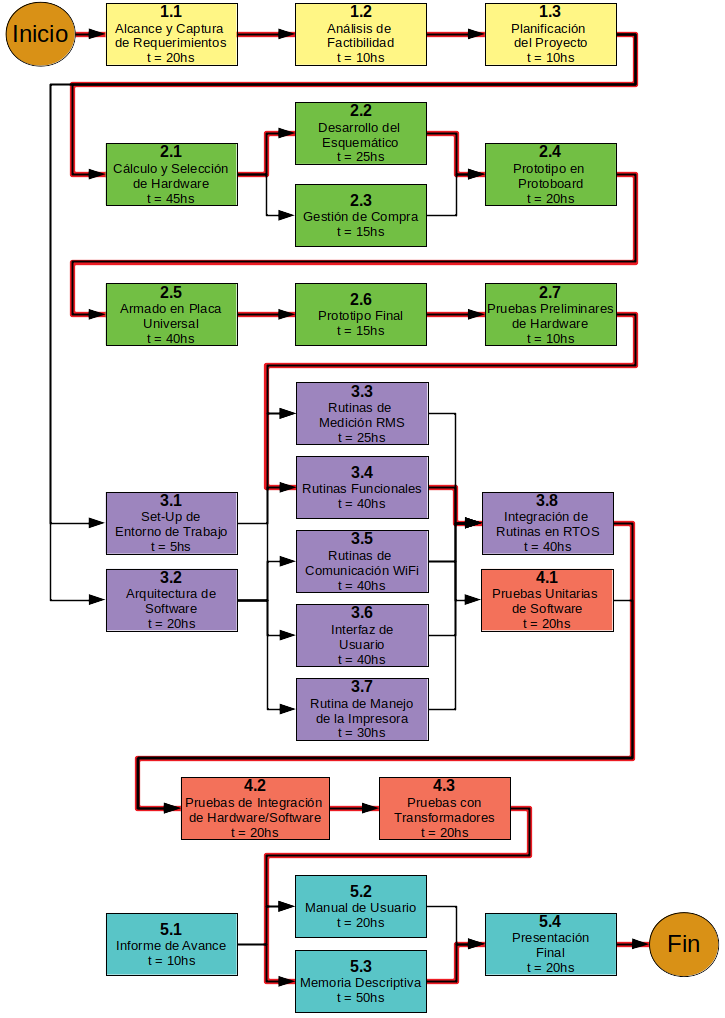
\includegraphics[width=.8\textwidth]{./Figuras/AoN.png}
\caption{Diagrama en \textit{Activity on Node}}
\label{fig:AoN}
\end{figure}



\begin{figure}[htpb]
\centering 
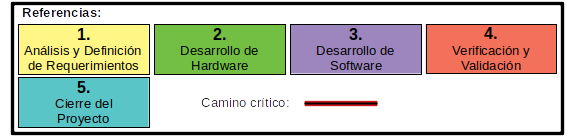
\includegraphics[width=.8\textwidth]{./Figuras/AoN_ref.png}
\caption{Referencias Diagrama en \textit{Activity on Node}}
\label{fig:AoN_ref}
\end{figure}


\newpage
\section{8. Diagrama de Gantt}
\label{sec:gantt}

\begin{figure}[htpb]
\centering 
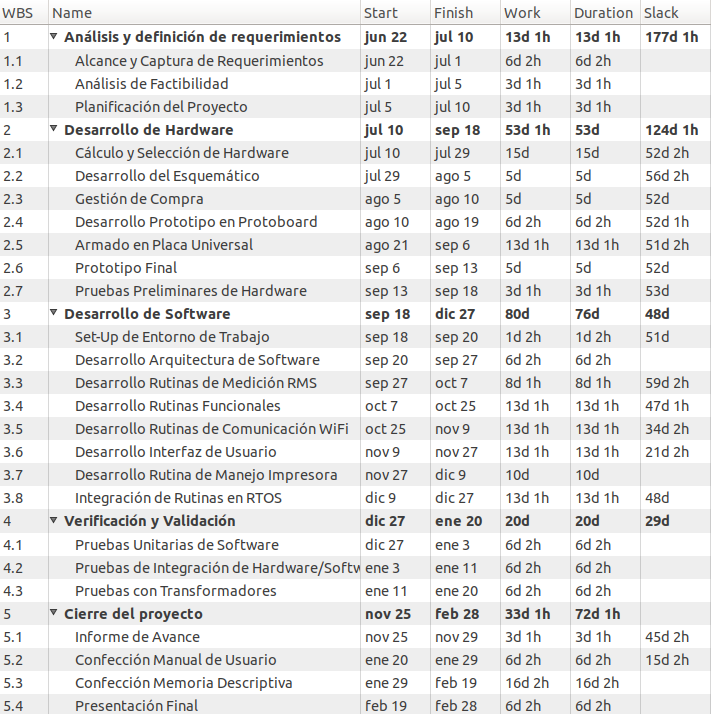
\includegraphics[width=.8\textwidth]{./Figuras/Gantt_1.png}
\caption{Diagrama de \textit{Gantt}}
\label{fig:Gantt_1}
\end{figure}


\begin{landscape}

\begin{figure}[htpb]
\centering 
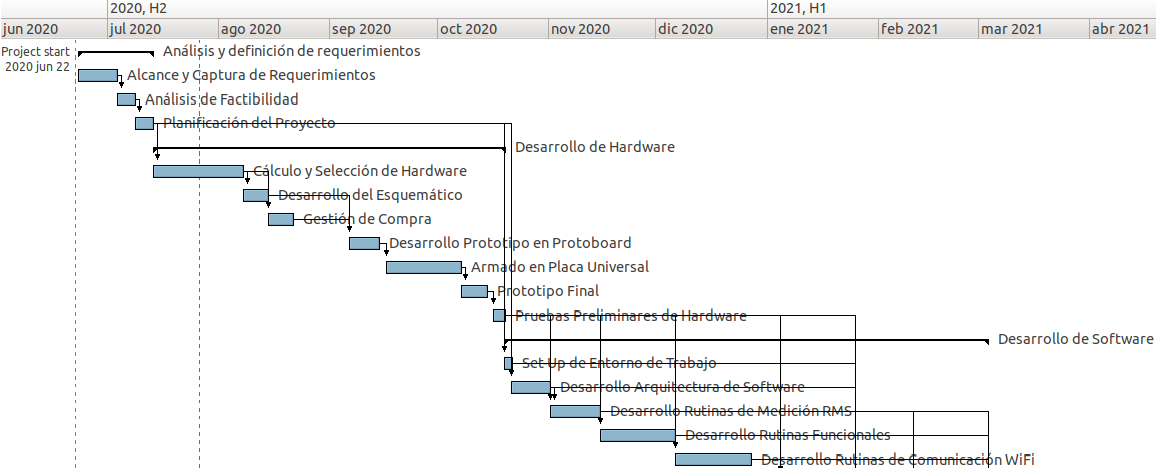
\includegraphics[width=1.57\textwidth]{./Figuras/Gantt_2.png}
\caption{Diagrama de \textit{Gantt} Cont.}
\label{fig:Gantt_2}
\end{figure}

\end{landscape}

\newpage

\begin{figure}[htpb]
\centering 
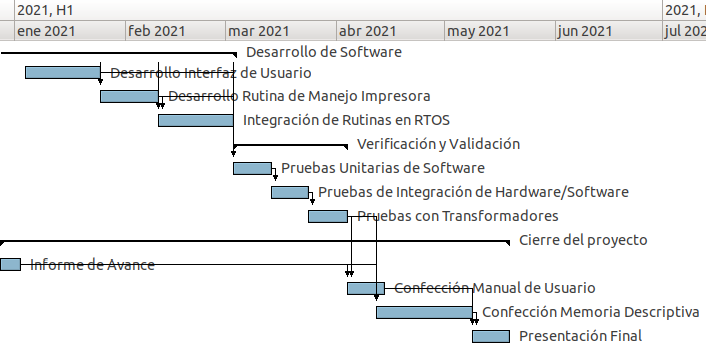
\includegraphics[width=.8\textwidth]{./Figuras/Gantt_3.png}
\caption{Diagrama de \textit{Gantt} Cont.}
\label{fig:Gantt_3}
\end{figure}

\section{9. Matriz de uso de recursos de materiales}
\label{sec:recursos}

\begin{table}[htpb]
\label{tab:recursos}
\centering
\begin{tabular}{|c|l|c|c|c|c|}
\hline
\cellcolor[HTML]{C0C0C0} & \multicolumn{1}{c|}{\cellcolor[HTML]{C0C0C0}{\color[HTML]{000000} }} & \multicolumn{4}{c|}{\cellcolor[HTML]{C0C0C0}Recursos requeridos (horas)}                                                                                                                                    \\ \cline{3-6} 
\multirow{-2}{*}{\cellcolor[HTML]{C0C0C0}\begin{tabular}[c]{@{}c@{}}Código\\ WBS\end{tabular}} & \multicolumn{1}{c|}{\multirow{-2}{*}{\cellcolor[HTML]{C0C0C0}{\color[HTML]{000000} \begin{tabular}[c]{@{}c@{}}Nombre\\ tarea\end{tabular}}}} & PC    & \begin{tabular}[c]{@{}c@{}}Equipamiento de \\ Laboratorio\end{tabular} & \begin{tabular}[c]{@{}c@{}}Prototipo\\ Protoboard\end{tabular} & \begin{tabular}[c]{@{}c@{}}Prototipo\\ Final\end{tabular} \\ \hline
1 & \begin{tabular}[c]{@{}l@{}}Análisis y definición\\ de Requerimientos\end{tabular} & 40  & & & \\ \hline
2 & Desarrollo de Hardware & 95  & 85 & 20 & 65 \\ \hline
3 & Desarrollo de Software & 240 & 100 & & 200 \\ \hline
4 & Verificación y Validación & 60  & 40 & & 60 \\ \hline
5 & Cierre del proyecto & 100 & 30 & & 30 \\ \hline
\end{tabular}
\end{table}

\newpage

\section{10. Presupuesto detallado del proyecto}
\label{sec:presupuesto}

\begin{table}[htpb]
\centering
\begin{tabularx}{\linewidth}{@{}|X|c|r|r|@{}}
\hline
\rowcolor[HTML]{C0C0C0} 
\multicolumn{4}{|c|}{\cellcolor[HTML]{C0C0C0}COSTOS DIRECTOS} \\ \hline
\rowcolor[HTML]{C0C0C0} 
Descripción &
  \multicolumn{1}{c|}{\cellcolor[HTML]{C0C0C0}Cantidad} &
  \multicolumn{1}{c|}{\cellcolor[HTML]{C0C0C0}Valor unitario} &
  \multicolumn{1}{c|}{\cellcolor[HTML]{C0C0C0}Valor total} \\ \hline
Placa de desarrollo ESP32 & \multicolumn{1}{c|}{1} & \multicolumn{1}{c|}{\$ 1620} & \multicolumn{1}{c|}{\$ 1620} \\ \hline
Sensor De Voltaje Alterna ZMPT101B 250V & \multicolumn{1}{c|}{2} & \multicolumn{1}{c|}{\$ 728} & \multicolumn{1}{c|}{\$ 1456} \\ \hline
Sensor De Corriente Alterna ZMCT103C & \multicolumn{1}{c|}{2} & \multicolumn{1}{c|}{\$ 1068} & \multicolumn{1}{c|}{\$ 2136} \\ \hline
Modulo Relé de 8 Canales & \multicolumn{1}{c|}{1} & \multicolumn{1}{c|}{\$ 1112} & \multicolumn{1}{c|}{\$ 1112} \\ \hline
\textit{Display} LCD \textit{Backlight} Azul 20x4 & \multicolumn{1}{c|}{1} & \multicolumn{1}{c|}{\$ 1140} & \multicolumn{1}{c|}{\$ 1140} \\ \hline
Fuente \textit{Switching} AC-DC 5 V 700 mA & \multicolumn{1}{c|}{2} & \multicolumn{1}{c|}{\$ 370} & \multicolumn{1}{c|}{\$ 740} \\ \hline
Modulo Conector MAX3232 & \multicolumn{1}{c|}{1} & \multicolumn{1}{c|}{\$ 320} & \multicolumn{1}{c|}{\$ 320} \\ \hline
Componentes varios & \multicolumn{1}{c|}{1} & \multicolumn{1}{c|}{\$ 1648} & \multicolumn{1}{c|}{\$ 1648} \\ \hline
Placa Experimental Doble Faz 9x15cm & \multicolumn{1}{c|}{1} & \multicolumn{1}{c|}{\$ 569} & \multicolumn{1}{c|}{\$ 569} \\ \hline
Horas de ingeniería & \multicolumn{1}{c|}{600} & \multicolumn{1}{c|}{U\$S 8} & \multicolumn{1}{c|}{U\$S 4960(*)} \\ \hline
\multicolumn{3}{|c|}{SUBTOTAL} &
  \multicolumn{1}{c|}{\$ 361241} \\ \hline
\rowcolor[HTML]{C0C0C0} 
\multicolumn{4}{|c|}{\cellcolor[HTML]{C0C0C0}COSTOS INDIRECTOS} \\ \hline 
\rowcolor[HTML]{C0C0C0} 
\multicolumn{3}{|l|}{Descripción} & \\ \hline
\multicolumn{3}{|l|}{Estimados como el 40\% de los costos directos} & \multicolumn{1}{c|}{\$ 144496} \\ \hline
\multicolumn{3}{|c|}{SUBTOTAL} &
  \multicolumn{1}{c|}{\$ 144496} \\ \hline
\rowcolor[HTML]{C0C0C0}
\multicolumn{3}{|c|}{TOTAL} & \multicolumn{1}{c|}{\$ 505737}
   \\ \hline
\end{tabularx}%
\end{table}

(*) 1 U\$S = 73 \$, cotización al día Jueves 23 de Julio 2020

\newpage

\section{11. Matriz de asignación de responsabilidades}
\label{sec:responsabilidades}

\begin{table}[htpb]
\centering
\resizebox{\textwidth}{!}{%
\begin{tabular}{|c|c|c|c|}
\hline
\rowcolor[HTML]{C0C0C0} 
\cellcolor[HTML]{C0C0C0} & \multicolumn{1}{c|}{\cellcolor[HTML]{C0C0C0}{\color[HTML]{000000} }} & \multicolumn{2}{c|}{\cellcolor[HTML]{C0C0C0}Listar todos los nombres y roles del proyecto} \\ \cline{3-4} 
\rowcolor[HTML]{C0C0C0} 
\multirow{-2}{*}{\cellcolor[HTML]{C0C0C0}\begin{tabular}[c]{@{}c@{}}Código\\ WBS\end{tabular}} & \multicolumn{1}{c|}{\multirow{-2}{*}{\cellcolor[HTML]{C0C0C0}{\color[HTML]{000000} \begin{tabular}[c]{@{}c@{}}Nombre\\ tarea\end{tabular}}}} & \begin{tabular}[c]{@{}c@{}}Responsable\\ \authorname \end{tabular} & \multicolumn{1}{c|}{\cellcolor[HTML]{C0C0C0}{\color[HTML]{333333} \begin{tabular}[c]{@{}c@{}}Orientador/Cliente\\ \clientename \end{tabular}}} \\ \hline
1.1 & Alcance y Captura de Requerimientos     & P & A \\ \hline
1.2 & Análisis de Factibilidad                & P &   \\ \hline
1.3 & Planificación del Proyecto              & P & C \\ \hline
2.1 & Cálculo y Selección de Hardware         & P & C \\ \hline
2.2 & Desarrollo del Esquemático              & P &   \\ \hline
2.3 & Gestión de Compra                       & P & A \\ \hline
2.4 & Desarrollo Prototipo en Protoboard      & P &   \\ \hline
2.5 & Armado en Placa Universal               & P &   \\ \hline
2.6 & Prototipo Final                         & P & C \\ \hline
2.7 & Pruebas Preliminares de Hardware        & P & I \\ \hline
3.1 & Set-Up de Entorno de Trabajo            & P &   \\ \hline
3.2 & Desarrollo Arquitectura de Software     & P &   \\ \hline
3.3 & Desarrollo Rutinas de Medición RMS      & P &   \\ \hline
3.4 & Desarrollo Rutinas Funcionales          & P &   \\ \hline
3.5 & Desarrollo Rutinas de Comunicación WiFi & P &   \\ \hline
3.6 & Desarrollo Interfaz de Usuario          & P & C \\ \hline
3.7 & Desarrollo Rutina de Manejo Impresora   & P & C \\ \hline
3.8 & Integración de Rutinas en RTOS          & P & I \\ \hline
4.1 & Pruebas Unitarias de Software           & P &   \\ \hline
4.2 & Pruebas de Integración de Hardware/Software & P & \\ \hline
4.3 & Pruebas con Transformadores             & P & I \\ \hline
5.1 & Informe de Avance                       & P & A \\ \hline
5.2 & Confección Manual de Usuario            & P & A \\ \hline
5.3 & Confección Memoria Descriptiva          & P & A \\ \hline
\end{tabular}%
}
\end{table}


{\footnotesize
Referencias:
\begin{itemize}
	\item P = Responsabilidad Primaria
	\item S = Responsabilidad Secundaria
	\item A = Aprobación
	\item I = Informado
	\item C = Consultado
\end{itemize}
} %footnotesize


\section{12. Gestión de riesgos}
\label{sec:riesgos}

a) Identificación de los riesgos y estimación de sus consecuencias:

Riesgo 1: posibilidad de no contar con pines de entrada/salidas suficientes.
\begin{itemize}
\item Severidad (S): 8. En caso de suceder podría no cumplirse con todos los requerimientos solicitados por el cliente.
\item Probabilidad de ocurrencia (O): 8. Muchas interfaces a conectar al ESP32 y este cuenta con 23 GPIOs. Habiendo hecho un conteo inicial de los pines y teniendo en cuenta que además de lo pedido se debe disponer de 4 pines más para JTAG, este evento tiene mucha probabilidad de ocurrir.
\end{itemize}  

Riesgo 2: daño o destrucción del hardware adquirido por el cliente.
\begin{itemize}
\item Severidad (S): 4. Los elementos de hardware utilizados están disponibles en el mercado local por lo que no se presentan dificultades para su obtención.
\item Probabilidad de ocurrencia (O): 5. Todo el conexionado en protoboard y armado de placa universal están a cargo del responsable del proyecto y se intentarán tomar las medidas necesarias para evitar fallos.
\end{itemize}

Riesgo 3: dificultad para conseguir el protocolo de comunicación de la impresora.
\begin{itemize}
\item Severidad (S): 7. En caso de ocurrencia implicaría perder la posibilidad de imprimir y es algo que el cliente desea mucho.
\item Probabilidad de ocurrencia (O): 5. No todos las fabricantes proveen código abierto para comunicarse con sus dispositivos.
\end{itemize}

Riesgo 4: no alcanzar la exactitud mínima de medición para las tensiones y/o corrientes de alterna.
\begin{itemize}
\item Severidad (S): 6. En caso de ocurrencia implicaría perder la posibilidad de discriminar algún tipo de transformador. 
\item Probabilidad de ocurrencia (O): 2. Se acotaron los errores a márgenes que pueden ser alcanzados con facilidad usando módulos estándar del mercado.
\end{itemize}

Riesgo 5: la comunicación WiFi afecta las mediciones analógicas.
\begin{itemize}
\item Severidad (S): 8. En caso de ocurrencia implicaría perder un poco de resolución en las mediciones analógicas. 
\item Ocurrencia (O): 7. El cliente comentó este efecto en una charla informal que se mantuvo con él.
\end{itemize}


b) Tabla de gestión de riesgos:

\begin{table}[htpb]
\centering
\begin{tabularx}{\linewidth}{@{}|X|c|c|c|c|c|c|@{}}
\hline
\rowcolor[HTML]{C0C0C0} 
Riesgo & S & O & RPN & S* & O* & RPN* \\ \hline
No contar con pines de entrada/salidas suficientes    & 8 & 8 &  \begin{consigna}{red}64\end{consigna} & 8  & 1  &  8   \\ \hline
Daño o destrucción del hardware adquirido por el cliente    & 4 & 5 &  20 &    &    &      \\ \hline
Dificultad para conseguir el protocolo de comunicación de la impresora    & 7 & 5 &  \begin{consigna}{red}35\end{consigna} & 7  & 1  &  7   \\ \hline
No alcanzar la exactitud mínima de medición para las tensiones y/o corrientes de alterna    & 6 & 2 &  12 &    &    &      \\ \hline
La comunicación WiFi afecta las mediciones analógicas    & 8 & 7 &  \begin{consigna}{red}56\end{consigna} & 8  & 1  &  8   \\ \hline
\end{tabularx}%
\end{table}

Criterio adoptado: se tomarán medidas de mitigación en los riesgos cuyos números de RPN sean mayores a 25.

Nota: los valores marcados con (*) en la tabla corresponden luego de haber aplicado la mitigación.

c) Plan de mitigación de los riesgos que originalmente excedían el RPN máximo establecido:
 
Riesgo 1: posibilidad de no contar con pines de entrada/salidas suficientes.

Plan de mitigación: se puede adquirir una interfaz serie I2C para conectar el \textit{display} al microcontrolador y de esta forma liberar los pines de este periférico, que por otro lado, es el que más pines ocupa.
\begin{itemize}
\item Severidad (S): 8. La severidad sigue siendo la misma.
\item Probabilidad de ocurrencia (O): 1. La probabilidad de ocurrencia baja al mínimo ya que se mitigó completamente el riesgo.
\end{itemize}

Riesgo 3: dificultad para conseguir el protocolo de comunicación de la impresora.

Plan de mitigación: se habló con el cliente la posibilidad de utilizar otras impresoras cuyos \textit{drivers} estén disponibles para ser implementados en un microcontrolador.
\begin{itemize}
\item Severidad (S): 7. La severidad sigue siendo la misma.
\item Probabilidad de ocurrencia (O): 1. La probabilidad de ocurrencia baja al mínimo ya que se mitigó completamente el riesgo.
\end{itemize}

Riesgo 5: la comunicación WiFi afecta las mediciones analógicas.

Plan de mitigación: instalar ADC externos.
\begin{itemize}
\item Severidad (S): 8. La severidad sigue siendo la misma.
\item Probabilidad de ocurrencia (O): 1. La probabilidad de ocurrencia baja al mínimo ya que se mitigó completamente el riesgo.
\end{itemize}

\section{13. Gestión de la calidad}
\label{sec:calidad}


\begin{itemize} 
\item Req \#1.1: el dispositivo debe ser diseñado en base al módulo ESP32.

Verificación y validación:

\begin{itemize}
\item Verificación: la planificación y el diseño debe estar basado en las características del módulo.
\item Validación: el prototipo final debe funcionar con el módulo ESP32, siendo este la unidad de procesamiento y transmisión.
\end{itemize}

\end{itemize}

\begin{itemize} 
\item Req \#1.2: el dispositivo debe ser capaz de medir tensiones y corrientes alternas de manera aislada del transformador bajo ensayo.

Verificación y validación:

\begin{itemize}
\item Verificación: se verificará que los módulos elegidos para las mediciones posean interfaces aisladas.
\item Validación: se realizaran ensayos con transformadores y elementos patrones para constatar las mediciones.  
\end{itemize}

\end{itemize}

\begin{itemize} 
\item Req \#1.3: el dispositivo debe ser capaz de conmutar las tensiones primarias y secundarias.

Verificación y validación:

\begin{itemize}
\item Verificación: se verificará que existan elementos de maniobra apropiados en el circuito.
\item Validación: se realizaran ensayos con transformadores y debe constatarse mediciones de corrientes en ambos bobinados al conmutar las tensiones.  
\end{itemize}

\end{itemize}

\begin{itemize} 
\item Req \#1.4: el dispositivo debe tener un \textit{display} LCD alfanumérico 20x4 caracteres.

Verificación y validación:

\begin{itemize}
\item Verificación: se verificará que exista dicho elemento en el circuito esquemático correctamente conectado al módulo ESP32.
\item Validación: al encender el equipo se deberán leer los valores correspondientes en dicho \textit{display}.  
\end{itemize}

\end{itemize}

\begin{itemize} 
\item Req \#1.5: el dispositivo debe tener una interfaz Wifi.

Verificación y validación:

\begin{itemize}
\item Verificación: se verificará que el módulo ESP32 posea dicha interfaz por medio de su hoja de datos. 
\item Validación: se verificará que el sistema envía/recibe los parámetros a través de una red WiFi al pulsar Configurar. 
\end{itemize}

\end{itemize}

\begin{itemize} 
\item Req \#1.6: el dispositivo debe tener una interfaz RS232 capaz de manejar impresoras.

Verificación y validación:

\begin{itemize}
\item Verificación: se verificará que exista dicha interfaz en el circuito esquemático correctamente conectado al módulo ESP32.
\item Validación: se conectará la interfaz a una impresora y se mandará a imprimir.
\end{itemize}

\end{itemize}

\begin{itemize} 
\item Req \#1.7: el dispositivo debe alimentarse desde la red eléctrica Argentina 220 Vac/50 hz, debiendo proveerse todas las alimentaciones a los diferentes módulos de hardware.

Verificación y validación:

\begin{itemize}
\item Verificación: se verificará que exista una fuente de 220 Vac que entregue las tensiones requeridas para el circuito.
\item Validación: se conectará el equipo a la red eléctrica y este debe funcionar. 
\end{itemize}

\end{itemize}

\begin{itemize} 
\item Req \#1.8: el dispositivo debe poseer un \textit{switch} para indicar que la tapa de seguridad ha sido removida.

Verificación y validación:

\begin{itemize}
\item Verificación: se verificará que exista dicho elemento en el circuito esquemático correctamente conectado al módulo ESP32.
\item Validación: se lanzará un proceso de caracterización en un transformador, luego se quitará la tapa de seguridad y se verificará que el equipo vaya a una condición segura.
\end{itemize}

\end{itemize}

\begin{itemize} 
\item Req \#1.9: el dispositivo debe poseer 3 pulsadores nombrados Configurar, Testear y Cancelar.

Verificación y validación:

\begin{itemize}
\item Verificación: se verificará que existan dichos elementos en el circuito esquemático correctamente conectado al módulo ESP32.
\item Validación: en las diferentes pruebas llevadas a cabo con el cliente estos pulsadores serán utilizados.
\end{itemize}

\end{itemize}

\begin{itemize} 
\item Req \#1.10: el dispositivo debe poseer un \textit{buzzer}.

Verificación y validación:

\begin{itemize}
\item Verificación: se verificará que exista dicho elemento en el circuito esquemático correctamente conectado al módulo ESP32.
\item Validación: se lanzará un proceso de caracterización en un transformador, y se verificará que al final de la prueba el \textit{buzzer} emita un zumbido.
\end{itemize}

\end{itemize}

\begin{itemize} 
\item Req \#2.1: requerimientos relativos a los valores a medir: bobinado primario

Verificación y validación:

\begin{itemize}
\item Verificación: se verificará mediante simulación analógica que los módulos seleccionados para dicha función cumplan con los rangos requeridos.
\item Validación: se colocarán los valores de tensiones correspondientes y estas y las corrientes generadas se deberán leer en el \textit{display} dentro de los rangos requeridos.
\end{itemize}

\end{itemize}

\begin{itemize} 
\item Req \#2.2: requerimientos relativos a los valores a medir: bobinado secundario

Verificación y validación:

\begin{itemize}
\item Verificación: se verificará mediante simulación analógica que los módulos seleccionados para dicha función cumplan con los rangos requeridos.
\item Validación: se colocarán los valores de tensiones correspondientes y estas y las corrientes generadas se deberán leer en el \textit{display} dentro de los rangos requeridos.
\end{itemize}

\end{itemize}

\begin{itemize} 
\item Req \#2.3: precisión en la medición de tensión: mejor al 1,5\% 

Verificación y validación:

\begin{itemize}
\item Verificación: se verificará mediante simulación analógica que los módulos seleccionados para dicha función cumplan con los rangos requeridos.
\item Validación: se colocarán los valores de tensiones correspondientes, estos se deberán leer en el \textit{display} y constatarse con algún elemento patrón acorde.  
\end{itemize}

\end{itemize}

\begin{itemize} 
\item Req \#2.4: precisión en la medición de corriente: mejor al 4\% 

Verificación y validación:

\begin{itemize}
\item Verificación: se verificará mediante simulación analógica que los módulos seleccionados para dicha función cumplan con los rangos requeridos.
\item Validación: se colocarán tensiones acordes en los bobinados para generar los valores de corrientes correspondientes, estos se deberán leer en el \textit{display} y constatarse con algún elemento patrón acorde.  
\end{itemize}

\end{itemize}

\begin{itemize} 
\item Req \#3.1: el dispositivo debe permitir que se configuren los umbrales mínimos y máximos para los parámetros medidos. 

Verificación y validación:

\begin{itemize}
\item Verificación: se comprobará que los umbrales mínimos y máximos sean variables y no constantes en el código C.
\item Validación: se configurarán los umbrales mínimos y máximos a través del procedimiento correspondiente.
\end{itemize}

\end{itemize}

\begin{itemize} 
\item Req \#3.2: los valores a configurar deben ser adquiridos solo por WiFi, no se admite configuración local por teclado.

Verificación y validación:

\begin{itemize}
\item Verificación: se comprobará que las rutinas de recepción WiFi incluyan la lectura de los umbrales mínimos y máximos.
\item Validación: se comprobará que el procedimiento de configuración de los umbrales mínimos y máximos, en el manual de usuario, es solo por WiFi. 
\end{itemize}

\end{itemize}


\begin{itemize} 
\item Req \#3.3: el dispositivo debe generar una confirmación de aceptación o rechazo del transformador en ensayo basado en los umbrales mínimos y máximos preseteados.

Verificación y validación:

\begin{itemize}
\item Verificación: se comprobará que las mediciones de las tensiones y corrientes de los transformadores se comparen con los umbrales seteados.
\item Validación: se lanzará un proceso de caracterización en un transformador con umbrales tales que generen la aceptación y el rechazo de este y se validarán los resultados.
\end{itemize}

\end{itemize}

\begin{itemize} 
\item Req \#3.4: el dispositivo, luego de cada ensayo, independientemente del resultado, debe imprimir una etiqueta con la siguiente información:
                \begin{enumerate}
                \item Número de partida del transformador ensayado
                \item Condición de aceptado o rechazado
                \item Valores medidos de tensiones y corrientes
                \end{enumerate}

Verificación y validación:

\begin{itemize}
\item Verificación: se comprobará, en la máquina de estado de la secuencia de testeo, que al finalizar el ensayo, dicha información sea enviada a la UART donde será conectada la impresora. 
\item Validación: se lanzará un proceso de caracterización en un transformador y se verificarán las etiquetas impresas.
\end{itemize}

\end{itemize}

\begin{itemize} 
\item Req \#3.5: el dispositivo debe seguir de forma automática la secuencia de testeo básico detallada en este requerimiento (se omite aquí por ser demasiados pasos).

Verificación y validación:

\begin{itemize}
\item Verificación: se comprobarán que exista la máquina estado para seguir dicho procedimiento.
\item Validación: se lanzará un proceso de caracterización en un transformador y se verificará dicha secuencia.  
\end{itemize}

\end{itemize}

\begin{itemize} 
\item Req \#4.1: solicitar parámetros de configuración: el dispositivo debe generar un comando GET de http a un servidor web (provisto por el cliente) para obtener los umbrales de aceptación y el número de partida del transformador a ensayar.

Verificación y validación:

\begin{itemize}
\item Verificación: se comprobarán la existencia  del comando GET de http en las APIs del módulo ESP32.
\item Validación: se pulsará Configurar y se verificará que los datos fueron correctamente obtenidos del servidor a través del \textit{display}.
\end{itemize}

\end{itemize}

\begin{itemize} 
\item Req \#4.2: el dispositivo debe ser capaz de procesar la respuesta del comando GET que estará en formato JSON.

Verificación y validación:

\begin{itemize}
\item Verificación: se comprobará la existencia de rutinas para procesar cadenas de tipo JSON.
\item Validación: se pulsará Configurar y se verificará que los datos fueron correctamente obtenidos del servidor a través del \textit{display}.
\end{itemize}

\end{itemize}

\begin{itemize} 
\item Req \#4.3: enviar resultados del ensayo: el dispositivo debe generar un comando POST de http a un servidor (provisto por el cliente) con la información del transformador ensayado en formato JSON.

Verificación y validación:

\begin{itemize}
\item Verificación: se comprobara la existencia del comando POST de http en las APIs del módulo ESP32. 
\item Validación: se lanzará un proceso de caracterización en un transformador y se comprobará que el servidor web recibe la información del transformador ensayado mostrada en el \textit{display}.
\end{itemize}

\end{itemize}

\begin{itemize} 
\item Req \#5.1.1: sobre la funcionalidad de los pulsadores - Configurar: al pulsar este pulsador el dispositivo debe generar el comando GET para solicitar al servidor web los parámetros de configuración del dispositivo a través de WiFi.

Verificación y validación:

\begin{itemize}
\item Verificación: se comprobará que la rutina de pulsado de Configurar llame el comando GET de http con la información requerida. 
\item Validación: se pulsará Configurar y se verificarán que los datos fueron correctamente obtenidos del servidor web corroborando su valor en el \textit{display}.
\end{itemize}

\end{itemize}

\begin{itemize} 
\item Req \#5.1.2: sobre la funcionalidad de los pulsadores - Testear: al pulsar este pulsador el dispositivo debe iniciar la secuencia de testeo.

Verificación y validación:

\begin{itemize}
\item Verificación: se comprobará, en la máquina de estado de la secuencia de testeo, que esta inicia cuando la tecla es pulsada.
\item Validación: se pulsará Testear y se verificará que comienza la secuencia de testeo básico descriptiva en el REQ 3.5 sección 4.
\end{itemize}

\end{itemize}

\begin{itemize} 
\item Req \#5.1.3: sobre la funcionalidad de los pulsadores - Cancelar: al pulsar este pulsador la secuencia de testeo en curso debe quedar abortada.

Verificación y validación:

\begin{itemize}
\item Verificación: se comprobará, en la máquina de estado de la secuencia de testeo, que esta aborta la secuencia cuando la tecla es pulsada.
\item Validación: se iniciará una rutina de testeo y se verificará que al pulsar Cancelar la secuencia de testeo es detenida. 
\end{itemize}

\end{itemize}

\begin{itemize} 
\item Req \#5.2.1: el dispositivo debe mostrar los umbrales configurados y los valores de las mediciones actuales.

Verificación y validación:

\begin{itemize}
\item Verificación: se comprobará que existan rutinas para mostrar dichos umbrales y mediciones en el \textit{display}.
\item Validación: se pulsará Configurar y se verificará en el \textit{display} los umbrales y mediciones.
\end{itemize}

\end{itemize}

\begin{itemize} 
\item Req \#5.2.2: los valores de los umbrales configurados en el dispositivo deberán permanecer en el \textit{display} durante el ensayo.

Verificación y validación:

\begin{itemize}
\item Verificación: se comprobará, en la máquina de estado de la secuencia de testeo, que los umbrales configurados son enviados al \textit{display} y que estos no son borrados del \textit{display} durante el ensayo.
\item Validación: se iniciará una rutina de testeo y se verificará que los umbrales configurados permanecen en el \textit{display} durante todo el ensayo.  
\end{itemize}

\end{itemize}

\begin{itemize} 
\item Req \#5.2.3: el dispositivo debe mostrar los valores medidos del transformador ensayado luego de cada medición.

Verificación y validación:

\begin{itemize}
\item Verificación: se comprobará, en la máquina de estado de la secuencia de testeo, que al finalizar cada medición los valores medidos son enviados al \textit{display}.
\item Validación: se iniciará una rutina de testeo y se verificará que los valores medidos del transformador ensayado son mostrados en el \textit{display} luego de cada medición.   
\end{itemize}

\end{itemize}

\begin{itemize} 
\item Req \#5.2.4: luego de finalizado el ensayo se debe mostrar un mensaje que indique que la información del ensayo se ha enviado al servidor web y mantenerse el dispositivo bloqueado hasta que se haya recibido la respuesta del servidor.

Verificación y validación:

\begin{itemize}
\item Verificación: se comprobará, en la máquina de estado de la secuencia de testeo, que la condición para finalizar el ensayo sea la recepción de la respuesta del web server.
\item Validación: se iniciará una rutina de testeo con el servidor no disponible y se verificará que el dispositivo permanece bloqueado.
\end{itemize}

\end{itemize}

\begin{itemize} 
\item Req \#5.3.1: el dispositivo debe emitir un solo sonido de 0,5 segundos de duración para confirmar la aceptación del transformador.

Verificación y validación:

\begin{itemize}
\item Verificación: se comprobará, en las rutinas de manejo del \textit{buzzer}, que cuando se levanta el \textit{flag} de "transformador aceptado", se genera un único pulso.
\item Validación: se iniciará una rutina de testeo con un transformados apto para ser aceptado y se verificará el sonido requerido.  
\end{itemize}

\end{itemize}

\begin{itemize} 
\item Req \#5.3.2: el dispositivo debe emitir un sonido de repetición de 5 ciclos de 0,5 segundos de duración, con pausas de 0,5 segundos para confirmar el rechazo del transformador.

Verificación y validación:

\begin{itemize}
\item Verificación: se comprobará, en las rutinas de manejo del \textit{buzzer}, que cuando se levanta el \textit{flag} de "transformador rechazado", se genera un tren de pulsos con las características adecuadas. 
\item Validación: se iniciará una rutina de testeo con un transformados apto para ser rechazado y se verificará el sonido requerido.   
\end{itemize}

\end{itemize}


\section{14. Comunicación del proyecto}
\label{sec:comunicaciones}

El plan de comunicación del proyecto es el siguiente:

% Please add the following required packages to your document preamble:
% \usepackage{graphicx}
% \usepackage[table,xcdraw]{xcolor}
% If you use beamer only pass "xcolor=table" option, i.e. \documentclass[xcolor=table]{beamer}
\begin{table}[htpb]
\centering
\resizebox{\textwidth}{!}{
\begin{tabular}{|c|c|c|c|c|c|}
\hline
\rowcolor[HTML]{C0C0C0} 
\multicolumn{6}{|c|}{\cellcolor[HTML]{C0C0C0}PLAN DE COMUNICACIÓN DEL PROYECTO}                                                                                                                                                                                              \\ \hline
\rowcolor[HTML]{C0C0C0} 
¿Qué comunicar? & Audiencia & Propósito & Frecuencia & Método de comunicac. & Responsable \\ \hline
\begin{tabular}[c]{@{}c@{}}Definición de los \\objetivos y los alcances\end{tabular} & Director  & Evaluar   & Inicio del Proyecto                                                    & Correo electrónico   & \begin{tabular}[c]{@{}c@{}}Cristian\\ Trinidad\end{tabular}  \\ \hline
\begin{tabular}[c]{@{}c@{}}Inicio de las tareas de \\ implementación\end{tabular}     & Director  & Informar  & \begin{tabular}[c]{@{}c@{}}Inicio de la \\ implementación\end{tabular} & Correo electrónico   & \begin{tabular}[c]{@{}c@{}}Cristian \\ Trinidad\end{tabular} \\ \hline
Grado de avance & Director  & Informar  & \begin{tabular}[c]{@{}c@{}}A la mitad del \\ proyecto\end{tabular}     & Correo electrónico   & \begin{tabular}[c]{@{}c@{}}Cristian \\ Trinidad\end{tabular} \\ \hline
\begin{tabular}[c]{@{}c@{}}Desvió de los alcances\\ y/o el cronograma\end{tabular}    & Director  & Informar  & Cuando surjan                                                          & Correo electrónico   & \begin{tabular}[c]{@{}c@{}}Cristian \\ Trinidad\end{tabular} \\ \hline
Finalización y Cierre                                                                 & Director  & Evaluar   & Final del Proyecto                                                     & Presentación         & \begin{tabular}[c]{@{}c@{}}Cristian \\ Trinidad\end{tabular} \\ \hline
\end{tabular}
}
\end{table}

\section{15. Gestión de Compras}
\label{sec:compras}

Los componentes que son necesarios comprar se pueden conseguir de forma local y no ameritan la redacción de un plan de compras. Por otro lado, esta tarea será llevada a cabo por el departamento de compras del cliente. Solo se seguirá un proceso informal con el cliente para estar seguro que todos los componentes requeridos llegan a destino.

En cuanto a la fabricación del prototipo, será realizado por el responsable del proyecto, por lo que no se necesitará gestión con proveedores de este servicio.

\newpage

\section{16. Seguimiento y control}
\label{sec:seguimiento}

\begin{table}[!htpb]
\centering
\begin{tabularx}{\linewidth}{@{}|c|X|X|X|X|X|@{}}
\hline
\rowcolor[HTML]{C0C0C0} 
\multicolumn{6}{|c|}{\cellcolor[HTML]{C0C0C0}SEGUIMIENTO DE AVANCE}                                                                       \\ \hline
\rowcolor[HTML]{C0C0C0} 
Tarea del WBS & Indicador de avance & Frecuencia de reporte & Resp. de seguimiento & Persona a ser informada & Método de comunic. \\ \hline
1.1 & Documento de Requerimiento aprobado & Al finalizar el documento & Cristian \newline Trinidad & Director & Correo electrónico \\ \hline
1.2 & Aceptación de todos los requerimientos & Semanal & Cristian \newline Trinidad & Director & Correo electrónico \\ \hline
1.3 & Porcentaje de planificación realizado & Semanal & Cristian \newline Trinidad & Profesores Gestión de Proyecto & Correo electrónico \\ \hline
2.1 a 2.2 & Cant. de módulos en esquemático & Al finalizar la tarea & Cristian \newline Trinidad & Director & Correo electrónico \\ \hline
2.3 & Módulos comprados & Semanal & Cristian \newline Trinidad & Director & Correo electrónico \\ \hline
2.4 a 2.7 & Diferentes módulos ensamblados & Semanal & Cristian \newline Trinidad & Director & Correo electrónico \\ \hline
3.1 & Programar el ESP32 & Al finalizar la tarea & Cristian \newline Trinidad & Director & Correo electrónico \\ \hline
3.2 & Doc. de Arquitectura aprobado & Semanal & Cristian \newline Trinidad & Director & Correo electrónico \\ \hline
3.3 - 3.7 & Diferentes rutinas funcionando & Semanal & Cristian \newline Trinidad & Director & Correo electrónico \\ \hline
3.8 & Diferentes rutinas intercambiando datos & Semanal & Cristian \newline Trinidad & Director & Correo electrónico \\ \hline
4.1 a 4.2 & Cant. de rutinas testeadas & Semanal & Cristian \newline Trinidad & Director & Correo electrónico \\ \hline
4.3 & Trafos validados & Semanal & Cristian \newline Trinidad & Director & Correo electrónico \\ \hline
5.1 a 5.3 & Cantidad de elementos del índice completos & Al finalizar el documento & Cristian \newline Trinidad & Director & Correo electrónico \\ \hline
5.4 & Trabajo Final presentado & Al finalizar la tarea & Cristian \newline Trinidad & Director & Correo electrónico \\ \hline
\end{tabularx}%%}
\end{table}


\section{17. Procesos de cierre}    
\label{sec:cierre}

\begin{itemize}
\item Pautas de trabajo a seguir para analizar si se respetó el Plan de Proyecto original:
\begin{itemize}
\item El cumplimiento de los requerimientos se validará con las pruebas de verificación y validación.
\item El correcto desglose de tareas y estimación de tiempos se evaluará con el diagrama de Gantt.
\item La estimación del presupuesto se evaluará comparando el dinero y horas hombre reales destinadas al proyecto y lo estimado oportunamente.
\item La correcta gestión de riesgos, en caso surgir algún riesgo identificado, se evaluará en función de si se mitigó según lo propuesto y la efectividad.
\end{itemize}
Responsable: Cristian Trinidad

\item Identificación de las técnicas y procedimientos útiles e inútiles que se utilizaron, y los problemas que surgieron y cómo se solucionaron. Este análisis será documentado y anexado al informe final del proyecto.

Responsable: Cristian Trinidad

\item Agradecimiento a las personas involucradas en el proyecto. Se invitará a la presentación pública del trabajo final al director y todos los colaboradores del proyecto.

Responsable: Cristian Trinidad

\end{itemize}



\end{document}
